%%%%%%%%%%%%%%%%%%%%%%%%%%%%%%%%%%%%%%%%%%
% Engineering problems / LaTeX Template
%		Semester 6
%		Institut d'Optique Graduate School
%%%%%%%%%%%%%%%%%%%%%%%%%%%%%%%%%%%%%%%%%%
%	6N-IntNum-BlocTraitImage	/ Image processing
%%%%%%%%%%%%%%%%%%%%%%%%%%%%%%%%%%%%%%%%%%
%
% Created by:
%	Julien VILLEMEJANE - 16/jul/2024
% Fichier.sty modifié pour changer la police de caractère
%	
%
%%%%%%%%%%%%%%%%%%%%%%%%%%%%%%%%%%%%%%%%%%
% Professional Newsletter Template
% LaTeX Template
% Version 1.0 (09/03/14)
%
% Created by:
% Bob Kerstetter (https://www.tug.org/texshowcase/) and extensively modified by:
% Vel (vel@latextemplates.com)
% 
% This template has been downloaded from:
% http://www.LaTeXTemplates.com
%
% License:
% CC BY-NC-SA 3.0 (http://creativecommons.org/licenses/by-nc-sa/3.0/)
%
%%%%%%%%%%%%%%%%%%%%%%%%%%%%%%%%%%%%%%%%%

\documentclass[a4paper,11pt,titlepage]{article} % The default font size is 10pt; 11pt and 12pt are alternatives

%%%%%%%%%%%%%%%%%%%%%%%%%%%%%%%%%%%%%%%%%%%%%%%%%%%%%%%%%%%%%%%%%%%%%%%%%%%%%%%%%%%%%%%%%%%%%%%%%%%%%%%%%%%%%%%%%%%%%%%%%%%%%%%%%%%%%%%%%%%%%%%%%%%%%%%%%%%%%%%%%%%%%%%%%%%%%%%%%%%%%%%%%%%%%%%%%%%%%%%%%%%%%%%%%%%%%%%%%%%%%%%%%%%%%%%%%%%%%%%%%%%%%%%%%%%%
\usepackage{opto_elec_villemejane}

%%%%%%%%%%%%%%%%%%%%%%%%%%%%%%%%%%%%%%%%%%%%%%%%
%%%%%%%%%%%%%%%%%%%%%%%%%%%%%%%%%%%%%%%%%%%%%%%%
\begin{document}



% Page de garde
\begin{titlepage}

\begin{center}
	\begin{minipage}{2.5cm}
	\begin{center}
		
\includegraphics[width=8cm]{images/Logo-LEnsE.png}
	\end{center}
\end{minipage}\hfill
\begin{minipage}{10cm}
	\begin{center}
	\textbf{Institut d'Optique Graduate School }\\[0.1cm]
    \textbf{Interfaçage Numérique}


	\end{center}
\end{minipage}\hfill


\vspace{4cm}


{\huge \bfseries \textsc{Interfaçage Numérique}} \\[0.5cm]
{\large \bfseries Travaux Pratiques} \\[0.2cm]
Semestre 6

\vspace{1.5cm}
% Title
\rule{\linewidth}{0.3mm} \\[0.4cm]
{ \huge \bfseries\color{violet_iogs} Images et OpenCV \\[0.4cm] }
\rule{\linewidth}{0.3mm} \\[0.2cm]
{ \large \bfseries\color{violet_iogs} Pré-traitements, masques, filtres et segmentation }
\rule{\linewidth}{0.3mm} \\[1cm]

2 séances

\bigskip

\begin{center}
	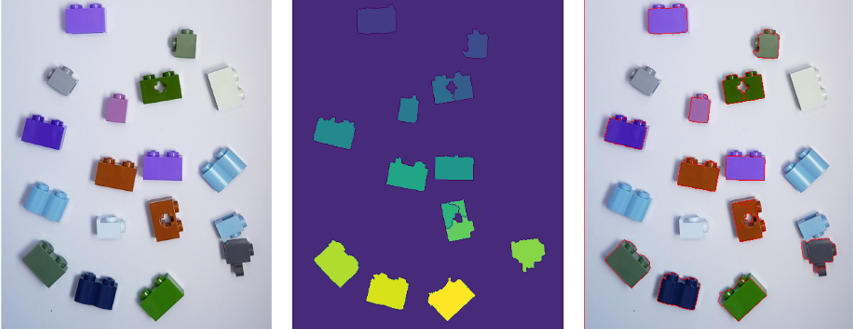
\includegraphics[width=0.8\textwidth]{images/trait_image.png}
\end{center}

\vfill

\textit{Ce sujet est disponible au format électronique sur le site du LEnsE - https://lense.institutoptique.fr/ dans la rubrique Année / Première Année / Interfaçage Numérique S6 / Bloc 2 Caméra, Images et Interfaces / Images et OpenCV.}


% Bottom of the page
%{\textbf{\large {Année universitaire} 2024-2025}}

\end{center}
\end{titlepage}

\newpage
\strut % empty page

\newpage
\pagestyle{empty}

\begin{minipage}[c]{.25\linewidth}
	
\includegraphics[width=5cm]{images/Logo-LEnsE.png}
\end{minipage} \hfill
\begin{minipage}[c]{.4\linewidth}

\begin{center}
\vspace{0.3cm}
{\Large \textsc{Interfaçage Numérique}}

\medskip

6N-047-SCI \qquad \textbf{\large Bloc Images/OpenCV}

\end{center}
\end{minipage}\hfill

\vspace{0.5cm}

\noindent \rule{\linewidth}{1pt}

{\noindent\Large  \rule[-7pt]{0pt}{30pt} \textbf{Images et OpenCV}}

\noindent \rule{\linewidth}{1pt}

\bigskip 

%%%%%%%%%%%%%%%%%%%%%%%%%%%%%%%%%%%%%%%%%%%%%%%%
%%%%%%%%%%%%%    A A V

{\large À l'issue des séances de TP concernant le \textbf{bloc de traitement d'images avec OpenCV}, les étudiant$\cdot$es seront capables d'utiliser OpenCV pour manipuler des images et appliquer des traitements simples : erosion/dilatation, filtres de lissage, masques...}

\medskip

%%%%%%%%%%%%%%%%%%%%%%%%%%%%%%%%%%%%%%%%%%%%%%%%
%%%%%%%%%%%%%    Ressources

\section{Ressources}

Un tutoriel sur les bases d'OpenCV est disponible à l’adresse suivante : 

\href{https://iogs-lense-training.github.io/image-processing/}{https://iogs-lense-training.github.io/image-processing/}

Un \textbf{kit d'images} est disponible sur le site du LEnsE dans la rubrique \textit{Année / Première Année / Interfaçage Numérique S6 / Bloc 2 Caméra, Images et Interfaces / Images et OpenCV / Kit d'images}. 

Des \textbf{fichiers de fonctions} sont disponibles sur le site du LEnsE dans la rubrique\textit{Année / Première Année / Interfaçage Numérique S6 / Bloc 2 Caméra, Images et Interfaces / Images et OpenCV / Répertoire vers codes à tester}. 


Quelques \textbf{exemples} et explications sur les différents pré-traitements d'images est disponible sur le site du LEnsE dans la rubrique \textit{Année / Première Année / Interfaçage Numérique S6 / Bloc 2 Caméra, Images et Interfaces / Images et OpenCV / Image Processing with OpenCV}. 

%%%%%%%%%%%%%%%%%%%%%%%%%%%%%%%%%%%%%%%%%%%%%%%%
%%%%%%%%%%%%%    Déroulement

\section{Déroulement du bloc}

\begin{description}
	\item[Etape 0 - 30 min] Ouvrir une image et faire son histogramme
	\item[Etape 1 - 30 min] Couleur vers niveau de gris
	\item[Etape 2 - 30 min] Seuillage et binarisation d'une image
	\item[Etape 3 - 60 min] Erosion, Dilatation et Gradient
	\item[Etape 4 - 90 min] Lissage du bruit
	\item[Etape 5 - 90 min] Isoler des éléments verticaux (ou horizontaux) dans une image grâce à des opérateurs morphologiques spécifiques
	\item[Etape 6 - 90 min] Détecter des contours et des points d'intérêt
	\item[Etape 7 - 90 min] Segmenter une image par la méthode de Watershed
	
\end{description}
	
	

\newpage
\section{Primitives}

En traitement d'image, les \textbf{primitives} sont les éléments fondamentaux ou les structures de base qui composent une image, sur lesquels des algorithmes peuvent opérer pour effectuer des analyses ou des traitements. 

Les primitives servent de \textbf{points de départ} pour la reconnaissance d'objets, l'analyse de scène, la segmentation d'image ou la reconstruction 3D. Par exemple, pour détecter un visage dans une image, l'algorithme peut commencer par identifier des primitives simples comme les yeux (points ou régions sombres), puis les relier pour former une structure cohérente.

\bigskip

On peut distinguer 3 catégories de primitives.

\subsection{Primitives de bas niveau}

Ce sont les entités les plus simples extraites directement des pixels de l'image. 

Par exemple :

\begin{itemize}
	\item Points : des pixels isolés ou des points d'intérêt
	\item Lignes ou segments : des ensembles de pixels alignés détectés par des algorithmes de détection de bord
	\item Contours : les frontières des objets définis par des changements d'intensité ou de couleur
	\item Régions : des groupes de pixels connectés ayant des propriétés similaires.
\end{itemize}


\subsection{Primitives de niveau intermédiaire}

Ces primitives sont obtenues en combinant ou en analysant les primitives de bas niveau. 

Par exemple :

\begin{itemize}
	\item Formes géométriques : rectangles, cercles, polygones
	\item Lignes ou segments : des ensembles de pixels alignés détectés par des algorithmes de détection de bord
	\item Objets simples : identification d'objets à partir de leurs contours ou formes.
\end{itemize}

\subsection{Primitives de haut niveau}

Ces primitives sont plus abstraites et dépendent de la compréhension sémantique de l'image. 

Par exemple :

\begin{itemize}
	\item Objets complexes : reconnaissance d'éléments comme des personnes ou des animaux
	\item Relations spatiales : liens entre différents objets (par exemple, un objet en avant d'un autre).
\end{itemize}



\newpage
%%%%%%%%%%%%%    Etape 0
\section{Ouvrir une image sous OpenCV et afficher son histogramme}

\begin{center} \textbf{\textit{Temps conseillé : 30 min}} \end{center}

\begin{mdframed}[style=sidebar,frametitle={}]
Notions : \href{https://iogs-lense-training.github.io/image-processing/contents/opencv.html#open-an-image}{\textit{Ouvrir une image}} - \href{https://iogs-lense-training.github.io/image-processing/contents/opencv.html#display-an-image
}{\textit{Afficher une image}} - \href{https://iogs-lense-training.github.io/image-processing/contents/opencv.html#enhance-the-image-contrast-and-brightness}{\textit{Calculer l'histogramme}}
\end{mdframed}
 
\Manip Créer un nouveau projet sous PyCharm et impoter la bibliothèque OpenCV2.

\Manip Ouvrir et afficher l'image \textsl{robot.jpg} du kit d'images fourni, en niveau de gris.

\Quest Quelle est la taille de l'image ? Quel est le type d'un élément ?

\Manip Calculer l'histogramme de l'image et l'afficher.

\medskip

\textit{Il peut être intéressant de \textbf{créer une fonction qui affiche automatiquement l'histogramme} d'une image à partir de ses données. Elle sera très utile dans la suite du TP pour voir l'impact des effets appliqués sur les images.}


%%%%%%%%%%%%%    Etape 1
\section{Couleur vers niveau de gris}

\begin{center} \textbf{\textit{Temps conseillé : 30 min}} \end{center}

\Manip Ouvrir et afficher l'image \textsl{couleurs\_4.png} du kit d'images fourni, au format RGB.

\Quest Quelle est la taille de l'image ? Quel est le type de données d'un élément ?


\Quest Est-il possible d'afficher un histogramme de l'image ? 

\Manip Créer une copie de la matrice image (fonction \textsl{copy()} de Numpy). 

\Manip Forcer à 0 tous les pixels du canal bleu de la copie de l'image et afficher la nouvelle image.


\subsection{RVB vs Niveau de gris}

Une image RVB contient 3 canaux (Rouge, Vert, Bleu ou \textit{RGB} en anglais), tandis qu'une image en niveaux de gris n'en a qu'un. Une image en niveau de gris sera \textbf{3 fois plus rapide} à analyser qu'une image en couleur RVB mais toute notion de couleur sera alors perdue.

\begin{center}
	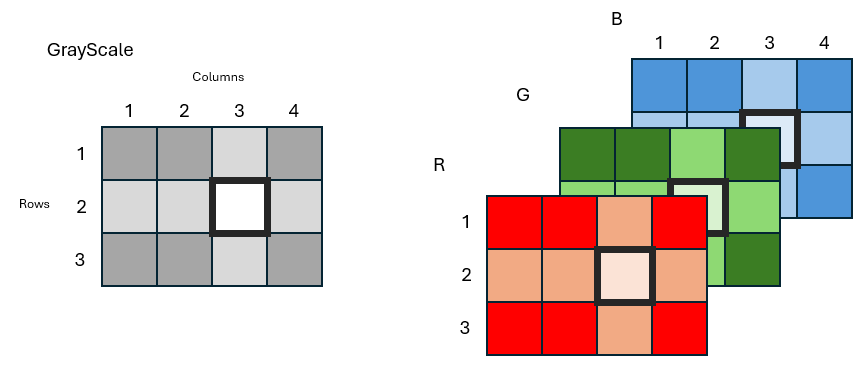
\includegraphics[width=0.8\textwidth]{images/images_array_gray_rgb.png}
\end{center}


La couleur des objets peut s'avérer inutile lorsqu'on cherche, par exemple, à détecter des formes particulières ou des contours dans une image.

De nombreux algorithmes d'analyse d'image ou de vision par ordinateur travaillent plus efficacement sur des images en niveaux de gris, permettant notamment d'uniformiser l'entrée des algorithmes et de réduire les informations redondantes liées à la couleur.

\subsection{Plusieurs méthodes de conversion}

Plusieurs méthodes existent pour passer d'une image RVB à une image en niveau de gris :

\begin{itemize}
	\item Calculer la \textbf{moyenne des valeurs} des trois canaux de couleur (Rouge, Vert, Bleu) pour chaque pixel.
	\item Utiliser des \textbf{poids spécifiques pour les canaux R, V et B}, basés sur leur contribution relative à la perception humaine.
	\item Convertir l'image dans un \textbf{autre espace de couleur}, comme YUV, HSL ou HSV, et extraire la composante de luminosité.
\end{itemize}

\subsubsection{Moyenne des canaux R,V,B}

Cette méthode est la plus simple. Chaque pixel de l'image en gris est la moyenne des pixels des canaux rouge, vert et bleu de l'image en couleur :

$$Pixel_{Gray} = \frac{Pixel_{R} + Pixel_{V} + Pixel_{B}}{3}$$ 

\Manip Créer une image en nuance de gris utilisant la méthode de la moyenne des trois canaux.

\Manip Afficher l'image résultante.


\subsubsection{Pondération en fonction de la perception humaine}

Cette méthode est une moyenne pondérée des valeurs des pixels R, V, B de l'image couleur : 

$$Pixel_{Gray} = 0.299 \cdot Pixel_{R} + 0.587 \cdot Pixel_{V} + 0.114 \cdot Pixel_{B}$$ 


Les coefficients de cette méthode proviennent de la sensibilité relative de l'œil humain aux différentes couleurs et ont été standardisés à l'origine pour la télévision analogique (NTSC). Ils sont aujourd'hui utilisés comme une approximation fidèle de la perception visuelle de la luminosité.

La méthode de conversion fournie par la bibliothèque OpenCV se base sur cette pondération.

\Manip Convertir l'image RVB en niveau de gris par l'instruction suivante :

\begin{lstlisting}
image_gray = cv2.cvtColor(image_rgb, cv2.COLOR_BGR2GRAY)
\end{lstlisting}

\Manip Comparer les images obtenues par la moyenne classique et cette moyenne pondérée.


\subsubsection{Utilisation d'un espace colorimétrique différent}

L'espace colorimétrique RVB est très utilisé dans le domaine du numérique (affichage, acquisition d'images) pour sa facilité de mise en oeuvre.

Cependant, ce n'est \textbf{pas} le plus \textbf{adapté vis-à-vis de la perception humaine} où la luminance et la couleur sont séparées.

Des espaces comme YUV, YIQ, ou YCbCr séparent la composante de luminance (Y) des composantes de chrominance (U et V).

\Manip Convertir l'image RVB dans l'espace YUV par l'instruction suivante :

\begin{lstlisting}
image_yuv = cv2.cvtColor(image_rgb, cv2.COLOR_RGB2YUV)
\end{lstlisting}

\Manip Comparer alors l'image en niveau de gris obtenue par la méthode de moyennage pondérée et le canal Y de cette conversion.

\Quest Que pouvez-vous conclure sur la méthode de calcul utiliser pour la luminance (Y) ?

\medskip

\noindent \rule{\linewidth}{1pt}

Il existe d'autres espaces colorimétriques dans le domaine numérique. Voici un résumé non exhaustif :

\begin{center}
\begin{tabular}{|c|c|}
\hline
\textbf{Espace colorimétrique} & \textbf{Avantages} \\ \hline
\textbf{RGB} & Simple, utilisé pour les écrans et le rendu des couleurs. \\ \hline
\textbf{HSV / HSL} & Intuitif pour manipuler la couleur (teinte, saturation). \\ \hline
\textbf{YUV / YCbCr} & Sépare luminance et chrominance. \\ \hline
\textbf{CIE-Lab} & Uniformité perceptuelle, idéal pour mesurer les différences de couleur. \\ \hline
\textbf{CMY(K)} & Optimisé pour l'impression. \\ \hline
\textbf{XYZ} & Modèle basé sur la perception humaine. \\ \hline
\end{tabular}
\end{center}

\newpage
%%%%%%%%%%%%%    Etape 2
\section{Seuillage et binarisation}

\begin{center} \textbf{\textit{Temps conseillé : 30 min}} \end{center}

\begin{mdframed}[style=sidebar,frametitle={}]
Notions : \href{https://iogs-lense-training.github.io/image-processing/contents/opencv.html#binarize-an-image}{\textit{Binarisation d'une image}} - \href{https://iogs-lense-training.github.io/python-for-science/contents/python_time.html}{\textit{Mesurer un temps d'exécution}}
\end{mdframed}

Le seuillage (ou binarisation) d'une image est une technique fondamentale en traitement d'image qui consiste à convertir une image en niveaux de gris en une image binaire, composée uniquement de deux niveaux (0 ou 1, ou encore noir et blanc).

\begin{center}
	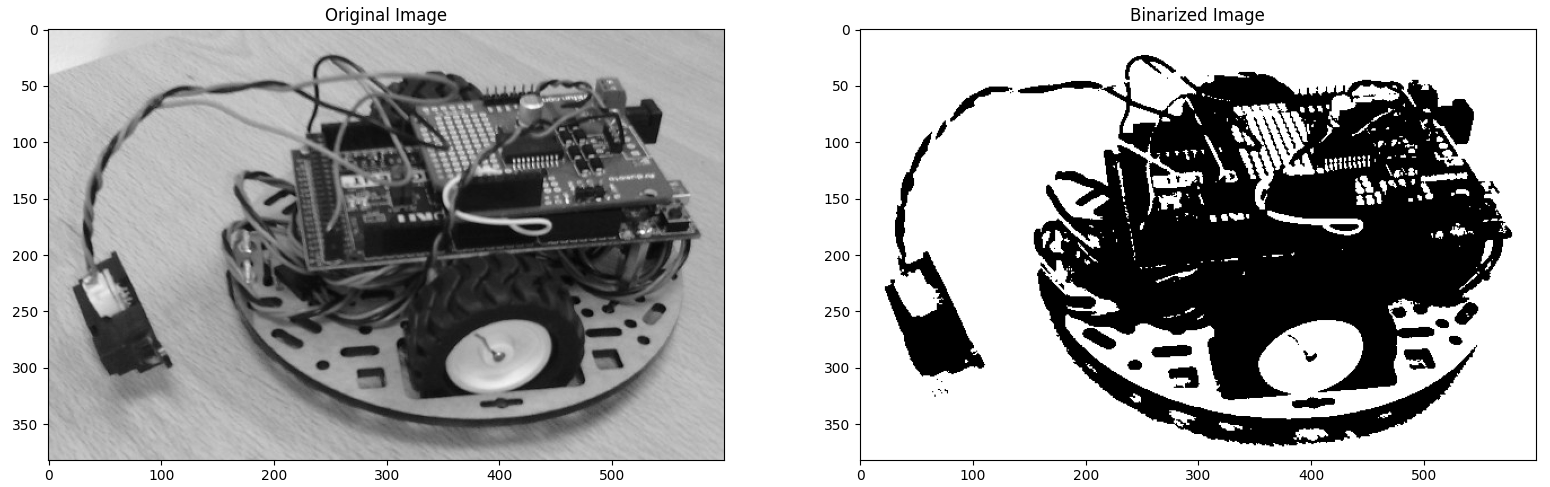
\includegraphics[width=0.8\textwidth]{images/binarized_image.png}
\end{center}

\subsection{Méthode classique}

\Manip Calculer l'image binarisée de l'image initiale - robot.jpg - (en niveau de gris) avec un seuil de 120, par la méthode \textsc{cv2.THRESH\_BINARY}.

\Manip Afficher l'image résultante. 

\Manip Tester également pour différente valeur de seuil. Tester également la méthode \textsc{cv2.THRESH\_BINARY\_INV}.

\Quest Que pouvez-vous conclure sur l'utilisation de cette méthode.

\subsection{Méthode d'Otsu}

La \textbf{méthode d'Otsu} permet d'effectuer un seuillage global automatique d'une image. Cette méthode est idéale pour les images où les niveaux de gris des objets et de l'arrière-plan forment \textbf{deux classes} bien distinctes. Dans ce cas, le seuil optimal pour séparer les niveaux de gris en deux classes (par exemple, objets d'intérêt et arrière-plan) est trouvé automatiquement : le seuil doit minimiser la variance intra-classe (dispersion des niveaux de gris dans chaque classe) et maximiser la variance inter-classe (différence entre les classes).

Cependant, son efficacité peut être limitée dans des cas de bruit ou de complexité multimodale.

\medskip

Il est possible d'utiliser cette méthode à l'aide de la fonction \textsl{threshold()} d'OpenCV de la façon suivante : 

\begin{lstlisting}
otsu_val, binary_image = cv2.threshold(image_gray, 0, 255, 
					cv2.THRESH_BINARY + cv2.THRESH_OTSU)
\end{lstlisting}

\Manip Tester cette méthode sur l'image \textbf{robot.jpg}. Comparer alors l'image résultante avec la méthode classique de seuillage.

\Quest A quoi correspond la valeur \textsl{otsu\_val} ?

\textit{Vous pourrez aussi comparer les temps d'exécution des deux méthodes...}


%%%%%%%%%%%%%    Etape 3
\section{Erosion, dilatation et gradient}

\begin{center} \textbf{\textit{Temps conseillé : 60 min}} \end{center}

On se propose ici d'analyser l'impact de différents procédés de pré-traitements (érosion, dilatation et gradient) sur une image.

\medskip

Les pré-traitements à étudier sont à réaliser sur l'image \textsl{a\_letter\_noise.jpg} du kit d'images fourni. Vous pourrez utiliser la fonction \textsl{zoom\_array()} fournie dans le fichier \textsl{images\_manipulation.py} afin d'augmenter la taille des images à analyser. 

\medskip

Pour faciliter l'analyse des images, on propose le code suivant permettant d'afficher 3 images en parallèle sur un même graphique :

\begin{lstlisting}
fig, ax = plt.subplots(nrows=1, ncols=3)    
ax[0].imshow(image_data_1, cmap='gray')
ax[0].set_title('Title Image 1')  
ax[1].imshow(image_data_2, cmap='gray')
ax[1].set_title('Title Image 2')
ax[2].imshow(image_data_3, cmap='gray')
ax[2].set_title('Title Image 3')
\end{lstlisting}


\subsection{Opérations de pré-traitement}

Les opérations de pré-traitement dans le traitement d'images sont essentielles pour \textbf{améliorer la qualité des images} avant d'appliquer des algorithmes plus complexes, comme la segmentation, la détection d'objets ou la classification. Ces étapes de pré-traitement visent à \textbf{réduire le bruit} ou \textbf{améliorer la structure de l'image}. 

Parmi les opérations de pré-traitement classiques, on peut citer :

\begin{itemize}
	\item \textbf{Correction des couleurs} : Balance des blancs, Correction gamma, Amélioration de contraste...
	\item \textbf{Réduction de bruit} : Filtrage linéaire pour atténuer les bruits sans trop affecter les détails importants de l'image, Filtrage non linéaire pour éliminer les bruits impulsionnels, Filtrage anisotrope...
	\item \textbf{Opérations morphologiques} : érosion pour éliminer du bruit, dilatation pour combler des lacunes dans les objets, ouverture et fermeture pour enlever les petites anomalies ou remplir les petits trous dans une image
	\item \textbf{Filtrage fréquentiel} pour éliminer ou atténuer des fréquences particulières (comme des motifs de bruit répétitifs) 
\end{itemize}

\subsection{Eléments structurants d'une convolution (noyau)}

\begin{mdframed}[style=sidebar,frametitle={}]
Notions : \href{https://iogs-lense-training.github.io/image-processing/contents/opencv_erod_dila.html#kernels-for-erosion-and-dilation}{\textit{Structuring Elements (kernels)}} 
\end{mdframed}

Les \textbf{transformations dites morphologiques} se basent sur l'application d'un \textbf{élément structurant} (ou noyau) que l'on va superposer sur chaque pixel de l'image. 

\Manip Générer un noyau en forme de croix de taille 3 par 3 pixels et afficher ce noyau.

\Quest Quel est le type de l'objet noyau résultant ?

\Manip Générer un second noyau en forme de carré de taille 3 par 3 pixels et afficher ce noyau.

\newpage
\subsection{Opérations d'érosion et de dilatation}

\begin{mdframed}[style=sidebar,frametitle={}]
Notions : \href{https://iogs-lense-training.github.io/image-processing/contents/opencv_erod_dila.html#erosion-operation}{\textit{Erosion}} - \href{https://iogs-lense-training.github.io/image-processing/contents/opencv_erod_dila.html#dilation-operation}{\textit{Dilation}} 
\end{mdframed}

\Manip Appliquer une opération d'érosion sur l'image \textsl{a\_letter\_noise.jpg} avec, indépendamment, les deux noyaux précédemment générés. 

\Manip Afficher les deux images ainsi que l'image originale sur un même graphique pour les comparer.

\Manip De la même manière, utiliser une opération de dilatation sur cette même image à l'aide des deux noyaux précédemment générés. Afficher également un comparatif des images résultantes.

\Quest Que pouvez-vous conclure sur l'utilité des opérations d'érosion et de dilatation sur une image ?

\subsection{Opérations d'ouverture et de fermeture}

\begin{mdframed}[style=sidebar,frametitle={}]
Notions : \href{https://iogs-lense-training.github.io/image-processing/contents/opencv_open_close.html#opening-operation}{\textit{Opening}} - \href{https://iogs-lense-training.github.io/image-processing/contents/opencv_open_close.html#closing-operation}{\textit{Closing}} 
\end{mdframed}

\Manip Appliquer une opération d'ouverture (\textit{opening}) sur l'image \textsl{a\_letter\_noise.jpg} avec, indépendamment, les deux noyaux précédemment générés. 

\Manip Afficher les deux images ainsi que l'image originale sur un même graphique pour les comparer.

\Manip De la même manière, utiliser une opération de fermeture sur cette même image à l'aide des deux noyaux précédemment générés. Afficher également un comparatif des images résultantes.

\Quest Que pouvez-vous conclure sur l'utilité des opérations d'ouverture et de fermeture sur une image ?

% L'opération d'opening est utile pour supprimer les petits bruits tout en maintenant la forme et la taille des objets plus grands dans l'image.


\subsection{Opération de gradient}

Une autre opération, appelée \textbf{gradient}, calcule la différence entre une dilatation et une érosion sur une même image. 

Il est possible de la mettre en pratique à l'aide de l'instruction suivante :

\begin{lstlisting}
gradient_image = cv2.morphologyEx(image, cv2.MORPH_GRADIENT, kernel)
\end{lstlisting}

\Manip Appliquer une opération de gradient sur l'image \textsl{robot.jpg} avec, indépendamment, les deux noyaux précédemment générés. 

\Manip Afficher les deux images ainsi que l'image originale sur un même graphique pour les comparer.

\Quest Que pouvez-vous conclure sur l'utilité de l'opération de gradient sur une image ?

% Le gradient met en évidence les bords des objets dans une image, ce qui peut être utile pour détecter des contours ou des transitions nettes dans l'intensité des pixels.

\newpage
%%%%%%%%%%%%%    Etape 4
\section{Lissage du bruit}

\begin{center} \textbf{\textit{Temps conseillé : 90 min}} \end{center}

\subsection{Générer du bruit sur des images}

On se propose d'étudier la fonction \textsl{generate\_gaussian\_noise\_image()} fournie dans le fichier 

\textsl{images\_manipulation.py}.

\Manip Tester l'exemple fourni dans le fichier \textsl{noise\_test1.py}.

\Quest Comment vérifier la distribution du bruit généré par cette fonction ?

\medskip

On se propose d'étudier la fonction \textsl{generate\_uniform\_noise\_image()} fournie dans le fichier 

\textsl{images\_manipulation.py}.

\Manip Tester l'exemple fourni dans le fichier \textsl{noise\_test2.py}.

\Quest La distribution du bruit généré par cette fonction est-elle uniforme ?

\Manip A l'aide de la fonction \textsl{generate\_gaussian\_noise\_image\_percent()}, générer un bruit gaussien de moyenne 30 et d'écart-type 20 sur 10\% de l'image \textsl{robot.jpg} ouverte précédemment en nuance de gris. 


\subsection{Comparer différents filtres de lissage}

On se propose à présent d'analyser l'impact de différents filtres de lissage  (flou gaussien, filtre médian et filtre moyenneur) sur une image.

Pour ces trois types de filtres, répéter les étapes suivantes :

\Manip Appliquer une opération de lissage avec le filtre souhaité sur l'image \textsl{robot.jpg} avec un noyau de 15 x 15 pixels.

\Manip Stocker dans une matrice la différence entre l'image originale et l'image lissée. Afficher l'image originale, l'image lissée et la différence de deux images sur un même graphique pour les comparer.

\Manip Ajouter du bruit gaussien sur l'image et appliquer à nouveau le filtre gaussien. Afficher l'image originale, l'image lissée et la différence de deux images sur un même graphique pour les comparer.

\Quest Que pouvez-vous conclure sur l'utilité d'un tel filtre ?

\textit{Vous pourrez également regarder l'impact de la taille du noyau sur l'image lissée finale.}


\subsubsection{Filtre de type gaussien}

\Manip Appliquer une opération de lissage de type \textsc{Gaussian Blur} sur l'image \textsl{robot.jpg} avec un noyau de 15 x 15 pixels (\textsl{cv2.GaussianBlur}).

\subsubsection{Filtre de type médian}

\Manip Appliquer une opération de lissage de type \textsc{Median Blur} sur l'image \textsl{robot.jpg} avec un noyau de 15 x 15 pixels (\textsl{cv2.medianBlur}).

\subsubsection{Filtre de type moyenneur (mean ou box)}

\Manip Appliquer une opération de lissage de type \textsc{Averaging Blur} sur l'image \textsl{robot.jpg} avec un noyau de 15 x 15 pixels (\textsl{cv2.blur}).


\newpage	
%%%%%%%%%%%%%    Etape 5
\section{Isoler des éléments d'une image grâce à des opérations linéaires}

\begin{center} \textbf{\textit{Temps conseillé : 90 min}} \end{center}

Les opérateurs d'érosion et de dilatation permettent d'extraire des informations particulières dans l'image à partir du moment où les éléments structurants (noyaux de convolution) sont judicieusement choisis.

On va chercher ici à détecter les lignes horizontales et verticales de l'image \textsl{\textit{forms\_opening\_closing.png}} :

\begin{center}
	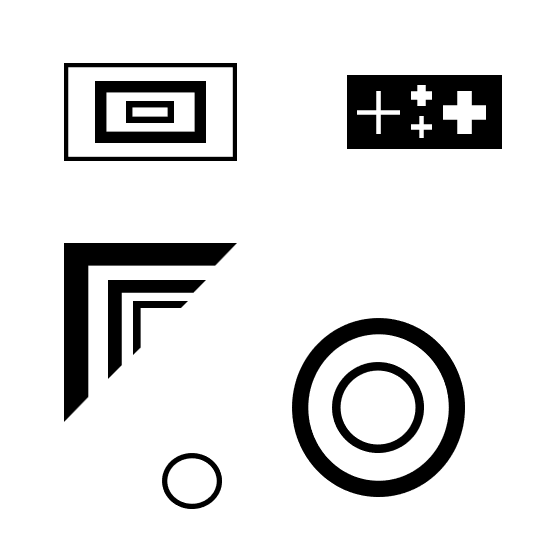
\includegraphics[width=0.4\textwidth]{images/forms_opening_closing_inv.png}
\end{center}


\Manip Tester l'exemple fourni dans le fichier \textsl{line\_detection.py}.

\Manip Afficher les images aux différentes étapes du traitement.

\Quest Analyser les différentes phases du traitement. Quelle est la forme du noyau utilisé ? Quel est l'impact de sa taille sur les éléments détectés ?

\Manip A partir de l'exemple précédent, écrire un script qui permet de détecter les lignes verticales de cette image et afficher le résultat.

\Manip Tester ces deux exemples sur d'autres images.


\newpage
%%%%%%%%%%%%%    Etape 6
\section{Détecter des contours et des points d'intérêt}

\begin{center} \textbf{\textit{Temps conseillé : 90 min}} \end{center}

Le traitement numérique des images, de manière automatisée, vise souvent à \textbf{extraire des informations} d'une image en se basant sur de la {détection des caractéristiques} très spécifiques (ou \textit{features detection}) : 

\begin{itemize}
	\item détection de coins (Harris...)
	\item détection de bords (Canny, Sobel, Prewitt...)
	\item détection de régions homogènes (Laplacien, Difference-of-Gaussian...)
	\item détection de lignes (Hough...)
\end{itemize}

Il existe également d'autres procédés plus complexes, notamment invariants à l'échelle et à la rotation, pour détecter des objets dans une image (SIFT, SURF, BRIEF...) ou basés sur l'apprentissage profond (R-CNN...).


\subsection{Détection de coins par la méthode de Harris}

Un \textbf{coin} est un point dans une image où l'\textbf{intensité change fortement dans plusieurs directions} (par opposition aux bords, où l'intensité change principalement dans une seule direction).

La \textbf{méthode de Harris} détecte ces coins en analysant les variations locales d'intensité des pixels. Elle repose sur une matrice appelée matrice de structure (ou matrice de Harris), qui résume la distribution locale des gradients dans une région autour d'un pixel. Cette matrice est définie comme suit :

$$M = \begin{pmatrix}
I_x^2 & I_x \cdot I_y \\
I_x \cdot I_y & I_y^2\\
\end{pmatrix}$$


où : $I_x$ et $I_y$ sont les dérivées partielles de l'intensité de l'image dans les directions $x$ et $y$. Ces dérivées sont calculées à l'aide d'un filtre Sobel ou similaire.


Pour chaque pixel, Harris calcule un score basé sur les valeurs propres ($\lambda_1$, $\lambda_2$) de $M$, en utilisant la formule suivante : 
$$R = det(M) - k \cdot (trace(M))^2$$
 
où : $det(M) = \lambda_1 \cdot \lambda_2$ est le déterminant de $M$, $trace(M) = \lambda_1 + \lambda_2$ est la trace de $M$ et $k$ est une constante (généralement entre 0.04 et 0.06).

Le score $R$ permet de distinguer les caractéristiques suivantes :

\begin{itemize}
	\item $R > 0$ : Coin (les deux directions présentent une variation significative) ;
	\item $R \approx 0$ : Région plate (pas de variation significative) ;
	\item $R < 0$ : Bord (variation dans une seule direction). 
\end{itemize}

\medskip

\Manip Ouvrir l'image \textsl{robot.jpg} du kit d'images fourni, en niveau de gris. 

\Manip Appliquer le code suivant sur l'image ainsi ouverte et afficher l'image résultante :

\begin{lstlisting}
image_harris = cv2.cornerHarris(image_gray, 2, 3, 0.04)
# result is dilated for marking the corners, not important
image_harris = cv2.dilate(image_harris, None)
# Threshold for an optimal value
image_gray[image_harris > 0.01 * image_harris.max()] = 0
\end{lstlisting}

\Manip Afficher également le résultat de la méthode \textsl{cornerHarris()}.

\Quest Que pouvez-vous conclure sur l'intérêt de la méthode de Harris ? Vous pourrez faire varier certains paramètres de la méthode \textsl{cornerHarris()}...


\subsection{Détection de contour par la méthode de Canny}

La méthode de Canny est un algorithme classique utilisé pour \textbf{détecter les bords} dans une image. On cherche ici à calculer des gradients d'intensité $G_x$ et $G_y$ pour estimer les changements d'intensité dans les directions horizontale et verticale (souvent à l'aide de filtres Sobel).

On peut alors définir l'amplitude du gradient $G$ et sa direction $\theta$ par les formules suivantes : 

$$G = \sqrt{G_x^2 + G_y^2}$$

$$\theta = arctan \frac{G_y}{G_x}$$

 
On souhaite ensuite ne conserver que les pixels correspondant aux crêtes (maxima locaux) des gradients dans la direction du gradient. Pour chaque pixel, on compare l'amplitude du gradient avec celles des pixels adjacents dans la direction $\theta$. Si ce n'est pas un maximum, le pixel est supprimé.

Puis deux seuils ($T_{haut}$ et $T_{bas}$) sont alors appliqués pour classifier les pixels :

\begin{itemize}
	\item $G > T_{haut}$ : pixels forts
	\item $T_{bas} < G < T_{haut}$ : pixels faibles
	\item $T_{bas} > G$ : pixels supprimés
\end{itemize}

Enfin, on détecte les pixels faibles qui sont connectés à des pixels forts. Ces ensembles sont conservés comme bords. Cela permet de relier les fragments de bords discontinus tout en éliminant les bords isolés ou bruités.

\medskip

\Manip Ouvrir l'image \textsl{robot.jpg} du kit d'images fourni, en niveau de gris. 

\Manip Appliquer le code suivant sur l'image ainsi ouverte et afficher l'image résultante :

\begin{lstlisting}
edges = cv2.Canny(image_gray, min_value, max_value)
\end{lstlisting}

\medskip

Pour en savoir plus sur l'algorithme de détection de contours de Harris : 

\href{https://docs.opencv.org/4.x/da/d22/tutorial_py_canny.html}{https://docs.opencv.org/4.x/da/d22/tutorial\_py\_canny.html} 


\newpage
%%%%%%%%%%%%%    Etape 7
\section{Segmenter une image par la méthode de Watershed}

\begin{center} \textbf{\textit{Temps conseillé : 90 min}} \end{center}

La méthode de \textbf{Watershed} (littéralement "ligne de partage des eaux") est une technique de \textbf{segmentation d'image} utilisée pour diviser une image en différentes régions ou objets. Elle est basée sur l'idée de traiter l'image comme une topographie où les niveaux de gris représentent des altitudes. L'objectif est de séparer les régions connectées tout en identifiant les limites précises entre elles.

Cette méthode nécessite au préalable quelques étapes de pré-traitement, basées sur les méthodes vues au cours de ce TP. 

L'algorithme complet, que vous allez mettre en oeuvre à présent, est le suivant :

\begin{enumerate}
	\item Ouverture de l'image en niveau de gris et seuillage (par la méthode d'Otsu)
	\item Réduction du bruit (ouverture morphologique)
	\item Identification des zones inconnues (ni fond, ni objets)
	\item Identification des objets	
	\item Application de l'algorithme de Watershed
\end{enumerate}

Pour le test et la compréhension de l'algorithme, il est intéressant d'afficher les images obtenues à chaque étape et de comprendre les différences avec l'étape précédente.
	
\subsection{Ouverture et seuillage}

\Manip Ouvrir l'image \textsl{bricks2.jpg} du kit d'images fourni, en niveau de gris. Puis appliquer un seuillage selon la méthode d'Otsu.

\subsection{Réduction du bruit}

\Manip Créer un élément structurant elliptique (\textsl{cv2.MORPH\_ELLIPSE}) de taille 3 par 3.

\Manip Utiliser ce noyau pour réaliser une opération morphologique d'ouverture sur l'image binaire précédemment obtenue. 

\subsection{Identification des zones inconnues}

Afin de pouvoir distinguer les objets sur l'image et ainsi les extraire du fond, nous allons chercher à séparer le fond (\textit{background}) des objets (\textit{foreground}).

\Manip Tester le code suivant sur l'image obtenue lors de l'étape précédente :

\begin{lstlisting}
# sure background area
sure_bg = cv2.dilate(opening, kernel, iterations=1)

# Finding sure foreground area
k_dist = 0.4
dist_transform = cv2.distanceTransform(opening, cv2.DIST_L1, 5)
ret, sure_fg = cv2.threshold(dist_transform, 
			k_dist * dist_transform.max(), 255, 0)

# Finding unknown region
sure_fg = np.uint8(sure_fg)
unknown = cv2.subtract(sure_bg, sure_fg)
\end{lstlisting}

\Quest A quoi correspondent les images : \textsl{sure\_bg}, \textsl{sure\_fg}, \textsl{unknown} et \textsl{dist\_transform} ?

\Quest Que se passe-t-il en modifiant le coefficient \textsl{k\_dist} ?

\subsection{Identification des objets}

Les pixels connectés dans les zones identifiées précédemment (\textsl{sure\_fg}) peuvent alors être considérés comme faisant partie d'un même objet. Il s'agit à présent de les identifier comme étant des objets différents.

\Manip Tester le code suivant sur l'image obtenue lors de l'étape précédente :

\begin{lstlisting}
# Marker labelling
ret, markers = cv2.connectedComponents(sure_fg)
# Add one to all labels so that sure background is not 0, but 1
markers = markers + 1
# Now, mark the region of unknown with zero
markers[unknown == 255] = 0
\end{lstlisting}

\Manip Afficher l'image \textsl{markers}.

\Quest A quoi correspond-elle ? La détection des objets est-elle optimale ? Pourquoi ?

\subsection{Application de l'algorithme de Watershed}

\Manip Tester le code suivant sur l'image obtenue lors de l'étape précédente (\textsl{markers}) et sur l'image RGB originale (\textsl{image\_rgb}) :

\begin{lstlisting}
image_rgb2 = image_rgb.copy()
markers2 = cv2.watershed(image_rgb, markers)
image_rgb[markers2 == -1] = [255, 0, 0]
\end{lstlisting}

\Quest A quoi sert la première ligne de ce code ?

\Manip Comparer l'image originale, l'image marquée par la méthode de Watershed et l'image finale.

\Quest Concluer sur l'intérêt d'un tel procédé et sur les paramètres qui peuvent modifier le résultat final.

%%%%%%%%%%%%%%%%%%%%%%%%%%%%%%%%%%%%%%%%%%%%%%%%
%%% RESSOURCES COMPLEMENTAIRES		

\newpage
\begin{center}
	\begin{minipage}{2.5cm}
	\begin{center}
		
\includegraphics[width=5cm]{images/Logo-LEnsE.png}
	\end{center}
\end{minipage}\hfill
\begin{minipage}{10cm}
	\begin{center}
	\textbf{Institut d'Optique Graduate School }\\[0.1cm]
    \textbf{Interfaçage Numérique}


	\end{center}
\end{minipage}\hfill


\vspace{2cm}


{\Large \bfseries \textsc{Interfaçage Numérique}} \\[0.5cm]
{\large \bfseries Travaux Pratiques} \\[0.2cm]
Semestre 6

\vspace{1cm}

% Title
\rule{\linewidth}{0.4mm} \\[0.4cm]
{ \Large \bfseries\color{violet_iogs} Ressources \\[0.4cm] }
\rule{\linewidth}{0.4mm} \\[1cm]
{\large Bloc Images et OpenCV}

\end{center}

\vspace{3cm}

\textbf{\large Liste des ressources}
\begin{itemize}
	\item \hyperref[doc:image_proc]{Image Processing / Key concepts}
\end{itemize}

\vfill

\newpage
\strut % empty page


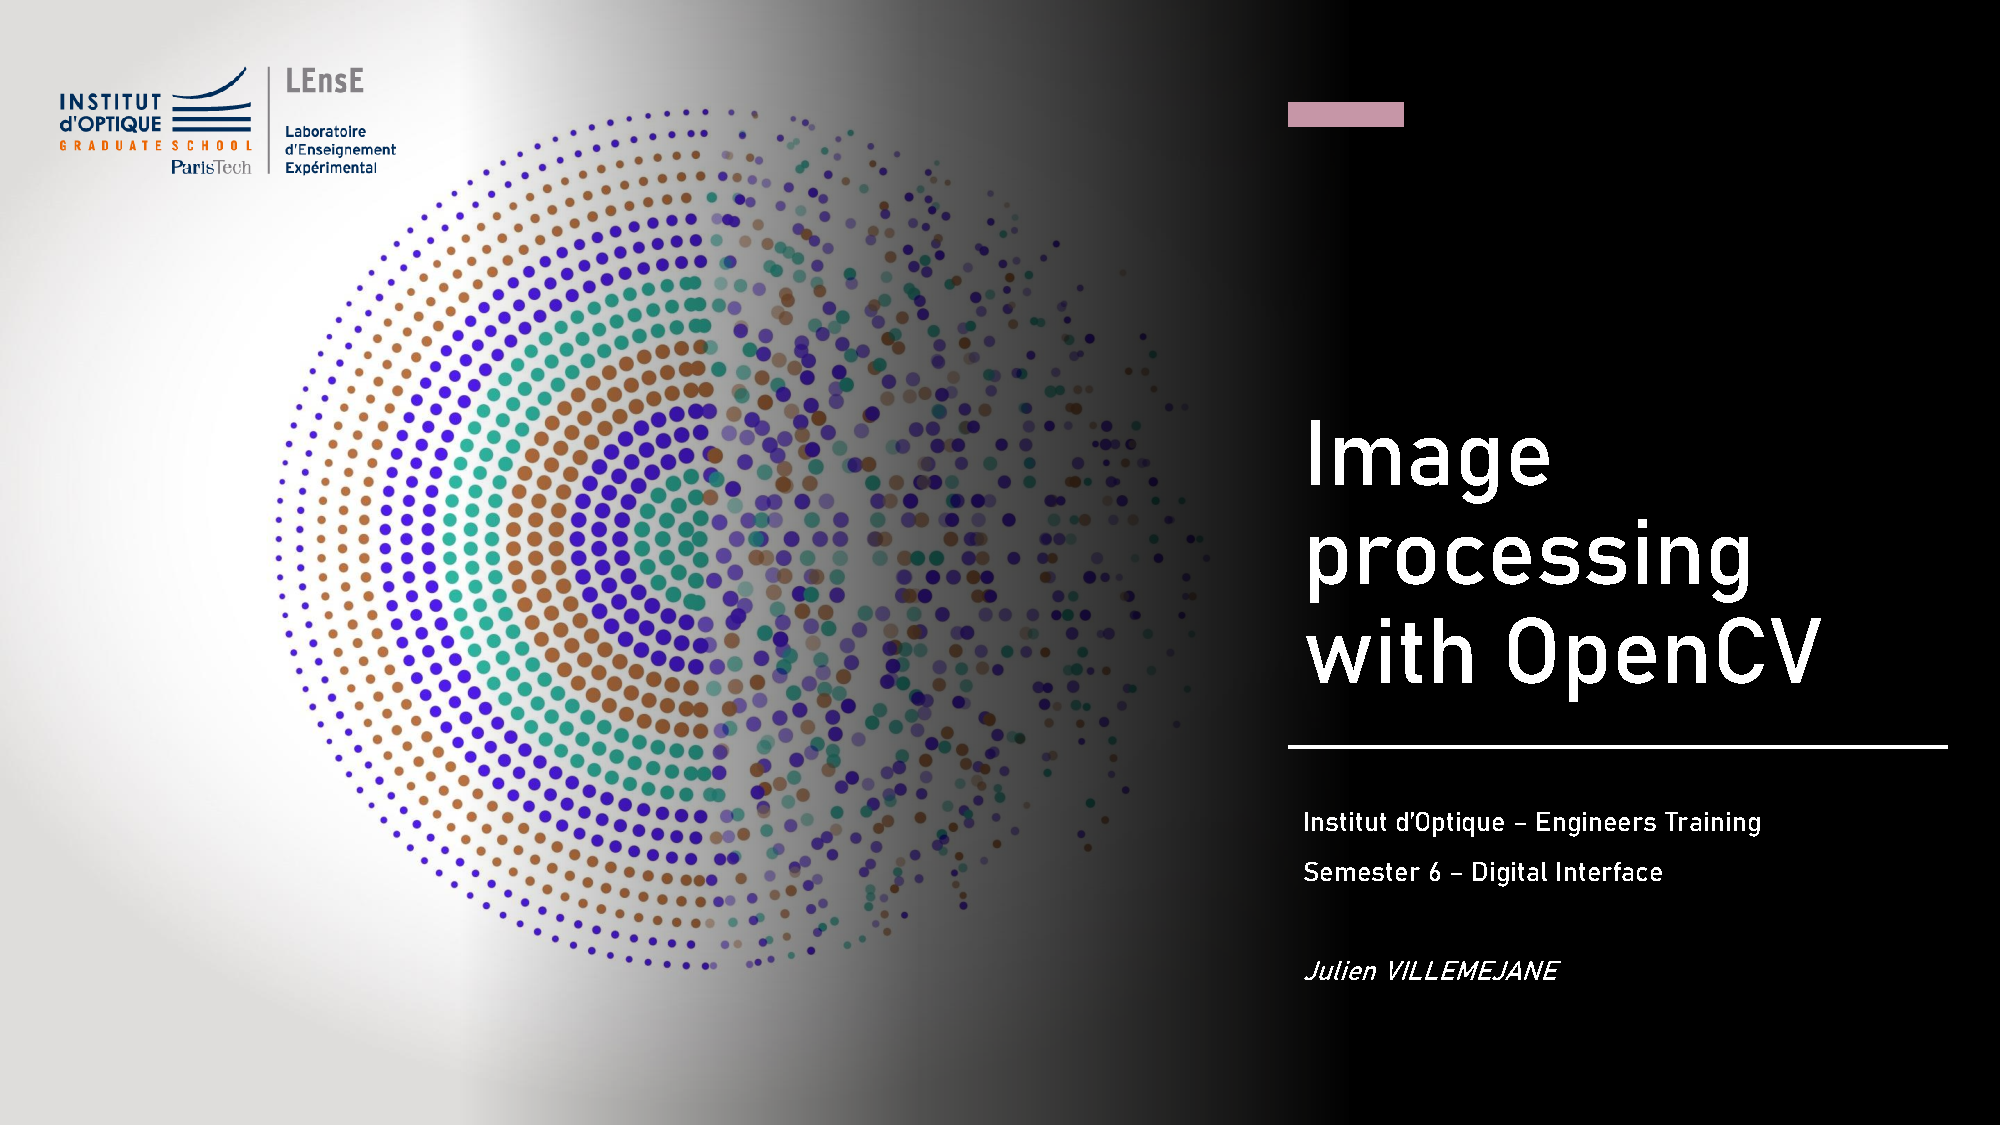
\includepdf[pages={1,4}, nup=1x2, pagecommand={\section{\texorpdfstring{\hspace{-1em}}{Image Processing}}}\label{doc:image_proc}]{../docs/Image_Processing.pdf}
\includepdf[pages={5,8,12,14,16,17,18,20,21,22,23,24,25,31}, nup=1x2]{../docs/Image_Processing.pdf}

\end{document}


